\section{Case Study}
\label{sec:case}

This case study, verification of a \textsf{post\_landing\_finalize} subsystem, is taken from an aircraft cabin pressure control application. The original Simulink model is from \href{https://www.honeywell.com/}{Honeywell} through our industrial link with \href{http://www.drisq.com/}{D-RisQ}. This case is also studied in \cite{Bhatt2016} and the diagram shown in Figure~\ref{fig:case} is from the paper. The purpose of this subsystem is to implement that the output $finalize\_event$ is triggered after the aircraft door has been open for a minimum specific amount of time following a successful landing. 

\begin{figure}[htb!]
    \begin{center}
        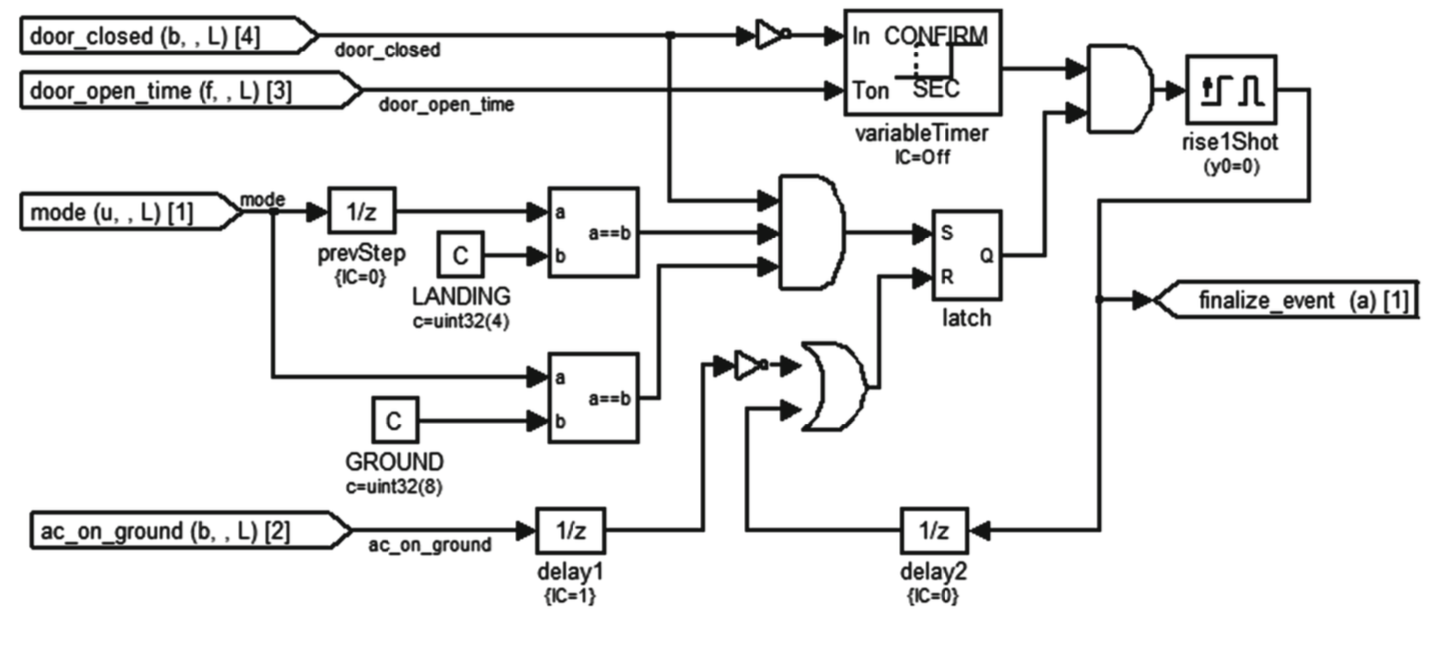
\includegraphics[scale=0.55]{postlanding}
    \end{center}
    \caption{Post Landing Finalize (source: \cite{Bhatt2016})}
    \label{fig:case}
\end{figure}

In order to apply our AG reasoning into this Simulink model, firstly we model the subsystem in our block theories as shown in Section~\ref{ssec:case_model}. Then we verify a number of properties for three small subsystems in this model, which is given in Section~\ref{ssec:case_veri}. Finally, in Section~\ref{ssec:case_req} we present verification of four requirements of this subsystem. To avoid confusion between the subsystem and three small subsystems, in the following sections we use the \emph{system} to denote the \textsf{post\_landing\_finalize} subsystem to be verified, and the \emph{subsystems} to denote three small subsystems.

\subsection{Modelling}
\label{ssec:case_model}

We start with translation of three small subsystems (\textsf{variableTimer}, \textsf{rise1Shot} and \textsf{latch}) according to our block theories. 

The subsystem \textsf{latch} is modelled as below. It is shown in Appendix~\ref{ssec:plf_latch} as well.
\begin{align*}
   & \left(\left(\left(\left((UnitDelay~0) \parallel_B Id\right) \dcomp (LopOR~2) \right) \parallel_B \left(Id \dcomp LopNOT\right) \right) \dcomp \left(LopAND~2\right) \dcomp Split2 \right)\ f_D\ (0,0) &
\end{align*}
The blocks $LopOR$, $LopNOT$ and $LopAND$ correspond to the OR, NOT and AND operators in the logic operator block. Their definitions can be found in Appendix~\ref{sec:block_theories}.  Then we apply composition definitions, expansion and SimBlock closure laws to simplify the subsystem. The \textsf{latch} subsystem is finally simplified to a design.
\begin{align*}
    & latch = FBlock \left( \logtrue{f}, 2, 1, latch\_simp\_pat\_f\right) &
\end{align*}
where the definition of $latch\_simp\_pat\_f$ is given in Appendix~\ref{sec:post_landing}. 

Similarly, \textsf{variableTimer} and \textsf{rise1Shot} are modelled and simplified as shown in Appendix~\ref{ssec:plf_variableTimer} and~\ref{ssec:plf_rise1Shot} respectively. 

Finally, we can use the similar way to compose the three subsystems with other blocks in this diagram to get the corresponding composition of \textsf{post\_landing\_finalise\_1}, and then apply the similar laws to simplify it further into one block and verify requirements for this system. However, for the outermost feedback it is difficult to use the similar way to simplify it into one block because it is more complicate than feedbacks in other three small subsystems (\textsf{variableTimer}, \textsf{rise1Shot} and \textsf{latch}). In order to use the expansion theorem~\ref{thm:fd_exp} of feedback, we need to find a solution for the block and prove the solution is unique. With increasing complexity of blocks, this expansion is becoming harder and harder. Therefore, \textsf{post\_landing\_finalise\_1} has not been simplified into one block. Instead, it is simplified to a block with a feedback which can be seen in the lemma \emph{post\_landing\_finalize\_1\_simp} in Appendix~\ref{sec:post_landing}.
\begin{align*}
  & post\_landing\_finalize\_1 = plf\_rise1shot\_simp\ f_D\ (4, 1) &
\end{align*}

\subsection{Subsystems Verification}
\label{ssec:case_veri}
After simplification, we can verify properties of the subsystems using the refinement relation. 

We start with verification of a property for \textsf{variableTimer}: \emph{vt\_req\_00}. This property states that if the door is closed, then the output of this subsystem is always false. The verification of this property is given in Appendix~\ref{ssec:plf_vt_veri}. However, this property can not be verified in absence of an assumption made to the second input: \emph{door\_open\_time}. This is due to a type conversion block \texttt{int32} used in the subsystem. If the input to \texttt{int32} is larger than $2147483647$ (that is, \emph{door\_open\_time} larger than $2147483647/10$), its output is less than zero and finally the output is true. That is not the expected result. Practically, \emph{door\_open\_time} should be less than $2147483647/10$. Therefore, we can make an assumption of the input and eventually verify this property as given in the lemma \emph{vt\_req\_00}. Additionally, we suggest a substitution of \texttt{int32} by \texttt{uint32}, or a change of the data type for the input from double to unsigned integer, such as \texttt{uint32}. 

As for the \textsf{rise1Shot} subsystem, we verified one property: \emph{rise1shot\_req\_00}. This property specifies that the output is true only when current input is true and previous input is false (see Appendix~\ref{ssec:plf_rise1shot_veri}). It means it is triggered only by a rising edge and continuous true inputs will not enable the output.

Furthermore, one property for the \textsf{latch} subsystem (a SR AND-OR latch) is verified (see Appendix~\ref{ssec:plf_latch_veri}). The property \emph{latch\_req\_00} states that as long as the second input $R$ is true, its output is always false. This is consistent with the definition of the SR latch in circuits.

\subsection{Requirement Verification}
\label{ssec:case_req}
The four requirements to be verified are illustrated in Table~\ref{tab:reqs}.
\begin{table}
    \centering
    \begin{tabular}{l|p{10cm}}
        \hline 
        Requirement 1 & A finalize event will be broadcast after the aircraft door has been open continuously for \emph{door\_open\_time} seconds while the aircraft is on the ground after a successful landing. \\
        \hline 
        Requirement 2 & A finalize event is broadcast only once while the aircraft is on the ground.\\
        \hline 
        Requirement 3 & The finalize event will not occur during flight. \\
        \hline 
        Requirement 4 & The finalize event will not be enabled while the aircraft door is closed. \\
        \hline
    \end{tabular}
    \caption{Requirements for the system (source: \cite{Bhatt2016})}
    \label{tab:reqs}
\end{table}

Our approach to cope with the difficulty to simplify this system into one design is to apply compositional reasoning. Generally, application of compositional reasoning to verify requirements is as follows.
\begin{itemize}
    \item In order to verify the property satisfied by \textsf{post\_landing\_finalise\_1}: \[C \refinedby post\_landing\_finalise\_1\], that is, to verify \[C \refinedby \left(plf\_rise1shot\_simp\ f_D\ (4, 1)\right)\];
    \item We need to find a decomposed contract $C'$ such that \[C \refinedby \left(C'\ f_D\ (4,1)\right)\] and \[\left(C' \refinedby plf\_rise1shot\_simp\right)\]; 
    \item Then we get \[\left(C'\ f_D\ (4,1)\right) \refinedby \left(plf\_rise1shot\_simp\ f_D\ (4, 1)\right)\] using the monotonicity theorem~\ref{thm:fd_mono} of feedback;
    \item Finally, according to transitivity of the refinement relation, it establishes that \[C \refinedby \left(plf\_rise1shot\_simp\ f_D\ (4, 1)\right)\].
\end{itemize}

\subsubsection{Requirement 3 and 4}
Requirement 3 and 4 are verified together as shown in Appendix~\ref{ssec:plf_req4}. $req\_04\_contract$ and $req\_04\_1\_contract$ are $C$ and $C'$ described above respectively. 

\subsubsection{Requirement 1}
According to Assumption 3 ``\emph{door\_open\_time} does not change while the aircraft is on the ground'' and the fact that this requirement specifies the aircraft is on the ground, therefore \emph{door\_open\_time} is constant for this scenario. In order to simplify the verification, we assume it is always constant. The contract $req\_01\_contract$ specifies that 
\begin{itemize}
  \item it always has four inputs and one output;
  \item and the requirement: 
     \begin{itemize}
        \item after a successful landing at step $m$ and $m+1$: the door is closed, the aircraft is on ground, and the mode is switched from LANDING (at step $m$) to GROUND (at step $m+1$),
        \item then the door has been open continuously for $door\_open\_time$ seconds from step $m+2+p$ to $m+2+p+door\_open\_time$, therefore the door is closed at the previous step $m+2+p-1$,
        \item while the aircraft is on ground: $ac\_on\_ground$ is true and $mode$ is GROUND,
        \item additionally, between step $m$ and $m+2+p$, the $finalize\_event$ is not enabled,
        \item then a $finalize\_event$ will be broadcast at step $m+2+p+door\_open\_time$.
     \end{itemize}
\end{itemize}

As shown in Appendix~\ref{ssec:plf_req1}, this requirement has been verified.

\subsubsection{Requirement 2}
The contract $req\_02\_contract$ specifies that 
\begin{itemize}
  \item it always has four inputs and one output;
  \item and the requirement: 
     \begin{itemize}
        \item if a finalize event has been broadcast at step $m$,
        \item while the aircraft is on ground: $ac\_on\_ground$ is true and $mode$ is GROUND,
        \item then a finalize event will not be broadcast again.
     \end{itemize}
\end{itemize}

As shown in Appendix~\ref{ssec:plf_req2}, this requirement has been verified too.

\subsection{Summary}
In sum, we have translated and mechanised the \textsf{post\_landing\_finalize} diagram in Isabelle/UTP, simplified its three subsystems (\textsf{variableTimer}, \textsf{rise1Shot} and \textsf{latch}) and the \textsf{post\_landing\_finalize} into a design with feedback, and finally verified all four requirements of this system. In addition, our work has identified a vulnerable block in \textsf{variableTimer}. This case study demonstrates that our verification framework has rich expressiveness to specify scenarios for requirement verification (as illustrated in the verification of Requirement 1 and 2) and our verification approach is useful in practice.
